\hspace{0.5 cm} Rezultatele obținute după rularea toolului alpha\textunderscore beta\textunderscore crown pe benchmark-ul cGAN au fost sub forma unui stream în consolă, dupa cum se vede în figura \ref{streamConsola}.

\begin{figure}[ht]
\centering
{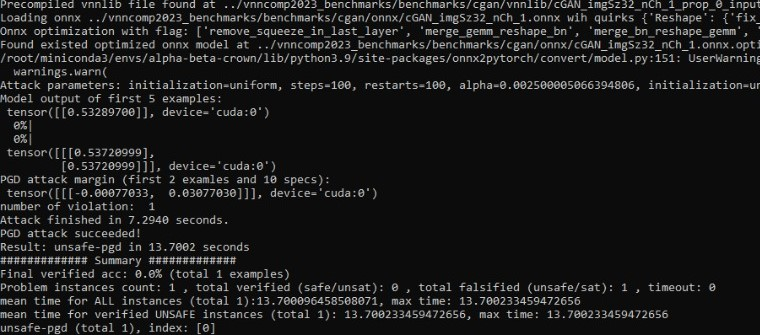
\includegraphics[width=15cm]{imagini/streamConsola.jpeg}}
\caption{Rezultat stream consola}
\label{streamConsola}
\end{figure}

Pentru a putea interpreta datele rezultate le-am clasificat manual într-un fișier excel. Câpurile de tabel sunt urmatoarele: 
\begin{itemize}
\item benchmark(benchmark-ul pentru care avem înregistrate rezultatele)

\item model\textunderscore neuronal(fișierul ONNX pentru care a rulat tool-ul)

\item specificații(fieșierul VNNLIB pentru care a rulat tool-ul)

\item rezultat(poate avea valori sat/unsat; sat înseamnă că modelul indeplinește condițiile din fișierul VNNLIB, adică distanța aproximată de discriminator, este aceeași cu distanța pe care a primit-o generator-ul ca și data de intrare; unsat înseamnă că discriminatorul nu a reușit să facă o aproximare corectă)

\item timp\textunderscore de\textunderscore verificare(timpul de rulare a fișierului ONNX pentru specificatiile din fișierul VNNLIB, exprimat în secunde). 
\end{itemize}

\href{https://docs.google.com/spreadsheets/d/1kSxunni8qgQLT6ZkCRWvSO2VMy2Hz7qA/edit#gid=1476783028}{Aici} se pot vedea rezultatele pe care le-am obținut.
Pentru a ne verifica corectitudinea rezultatelor obținute, am facut o analiză comparativă între fișierul obținut la rularea noastră, \href{https://docs.google.com/spreadsheets/d/1kSxunni8qgQLT6ZkCRWvSO2VMy2Hz7qA/edit#gid=1476783028}{aici}, și cel obținut din competiție, \href{https://drive.google.com/file/d/1XolWcngRIGwjblvrm2a5FD2AqH8fVWgt/view?usp=drive_link}{aici}. 


Am observat că pentru fiecare intrare, în ambele fișiere, s-a obținut același rezultat(sat/unsat). O diferență dintre cele două fișiere o constituie coloana ce reprezinta timpul de verificare. Am remarcat că în fișierul obținut de noi, timpul de verificare înregistrat este mai mic cu aproximativ 3 secunde pentru intrările unde rezultatul este satisfiabil. În schimb, pentru intrările cu rezultat nesatisfiabil timpul de verificare este considerabil mai mare.